The results of the \textit{Drawing Study} are presented separately for Task 1 and 4, but Task 2 and 3 share a single table. Originally the study design was meant to lead to four sketches per participant, but since Task 3 built up on the previous one, it only led to verbal comments by our participants or just slight modifications to the existing sketches from Task 2. This means every study session led to three sketches instead of four.

\subsection*{Task 1}
An overview of the results of Task 1 can be found in Table \ref{tb:t1}. The first row and column list categories, while the numbers in the table are the sums of sketches that fall into this category. If a sketch matches the \textbf{Explicit...} category, it also falls into at least one of the categories of the first column, since these describe in which way the uncertainty was represented explicitly. The individual categories are described in the following list:

\begin{itemize}
	\item \textbf{Graph} Sketches that count towards this category feature some kind of conventional line graph. Figure \ref{fig:graph} shows an example sketch, that fits this category. It is also important to notice that every graph visualization also counts toward the \textbf{Explicit...} category and \textit{...Length/Height} sub-category.
	
	\begin{figure}[H]
		\begin{minipage}{.5\textwidth}
			\centering
			\captionsetup{width=0.8\textwidth}
			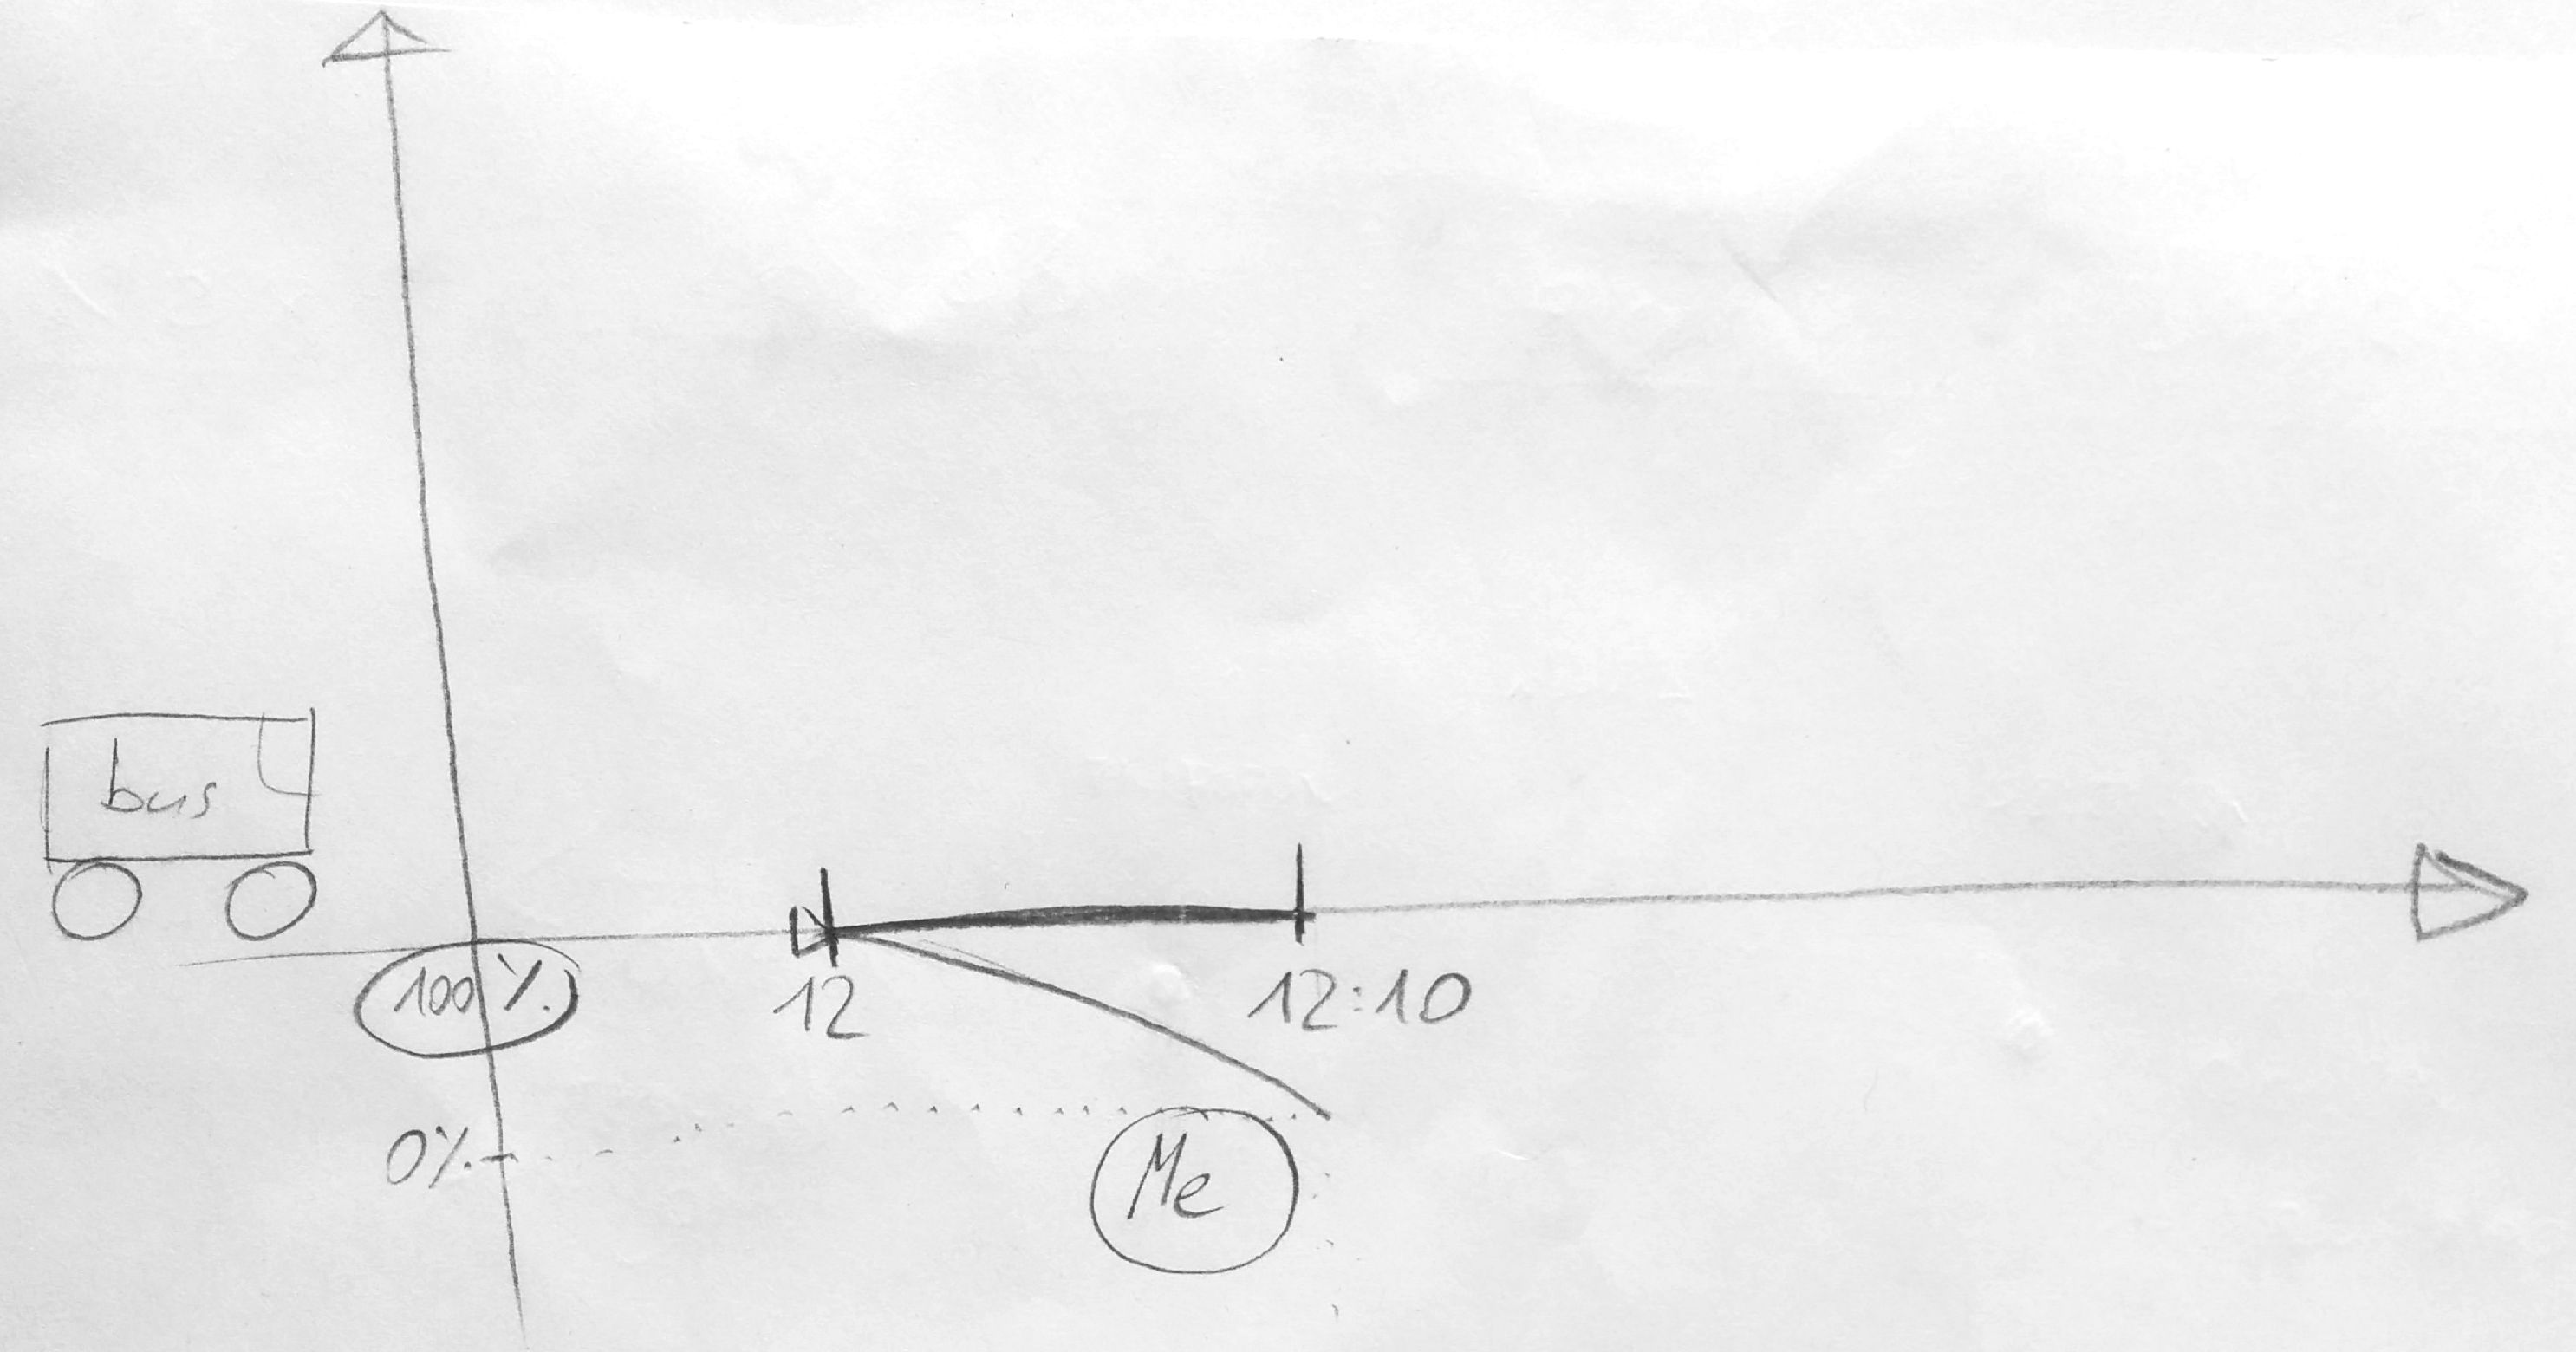
\includegraphics[height=0.5\textwidth]{figures/graph.jpg}
			\caption{\textit{This conventional graph visualization shows the probability of reaching the bus over a given time interval.}}
			\label{fig:graph}
		\end{minipage}
		\begin{minipage}{.45\textwidth}
			\centering
			\captionsetup{width=1.0\textwidth}
			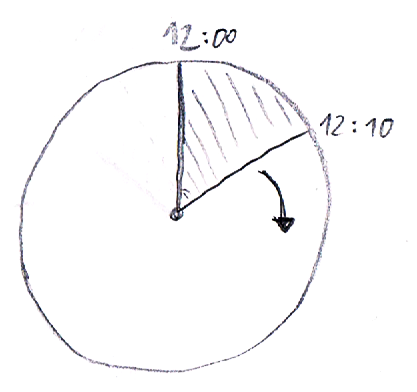
\includegraphics[height=0.5\textwidth]{figures/clock.png}
			\caption{\textit{The clock metaphor used in this visualization quickly makes clear, that temporal data is presented. In this case the uncertainty is only given through the bounds of the uncertainty interval.}}
			\label{fig:clock}
		\end{minipage}
	\end{figure}
	
	\item \textbf{Clock} As shown in Figure \ref{fig:clock}, some participants utilized a clock metaphor to visualize time intervals.
	
	\item \textbf{Explicit...} A sketch counts towards this category, if the uncertainty for a given point in time is somehow represented explicitly, instead of just by the relative position to the bounds of the uncertain time frame. To further split up this category, the following four sub-categories describe the way the uncertainty is represented. Sometimes multiple representations were used in combination, which is why the sum of sub-category counts do not add up to the total number of explicitly represented uncertainties. Figure \ref{fig:explicit} shows an example for every sub-category.
	\begin{itemize}
		\item \textit{...Icons} This means that the uncertainty for a given point in time was represented by an icon. Often smileys were used for this type of encoding.
		\item \textit{...Color} This means that the uncertainty was represented by a color value. This could for instance be a color gradient from one color, representing uncertainty, to another color, representing certainty. 
		\item \textit{...Length/Height} This means that the uncertainty was given through position of something (e.g. a line). A common example would be a conventional line graph that represents values through the height of a line at a given point.
		\item \textit{...Interaction} Sometimes the uncertainty of a given point in time was directly stated in a percentage value. To find out about the probabilities of different time points, user interaction was needed.
		
		\begin{figure}[h]
			\begin{subfigure}[t]{.4\textwidth}
				\centering
				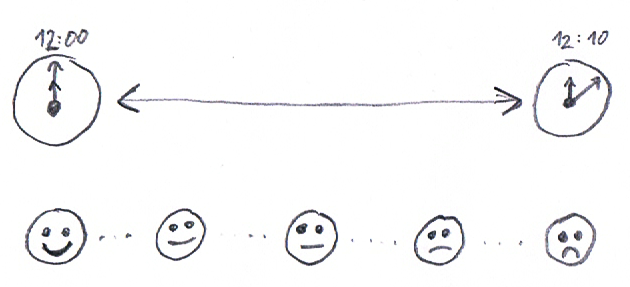
\includegraphics[width=\linewidth]{figures/icons.png}
				\caption{\textit{The clock represent the relevant interval, while the uncertainty over this interval is encoded in smiley faces of varying happiness.}}
				\label{fig:icons}
			\end{subfigure}
			\hfill
			\begin{subfigure}[t]{.4\textwidth}
				\centering
				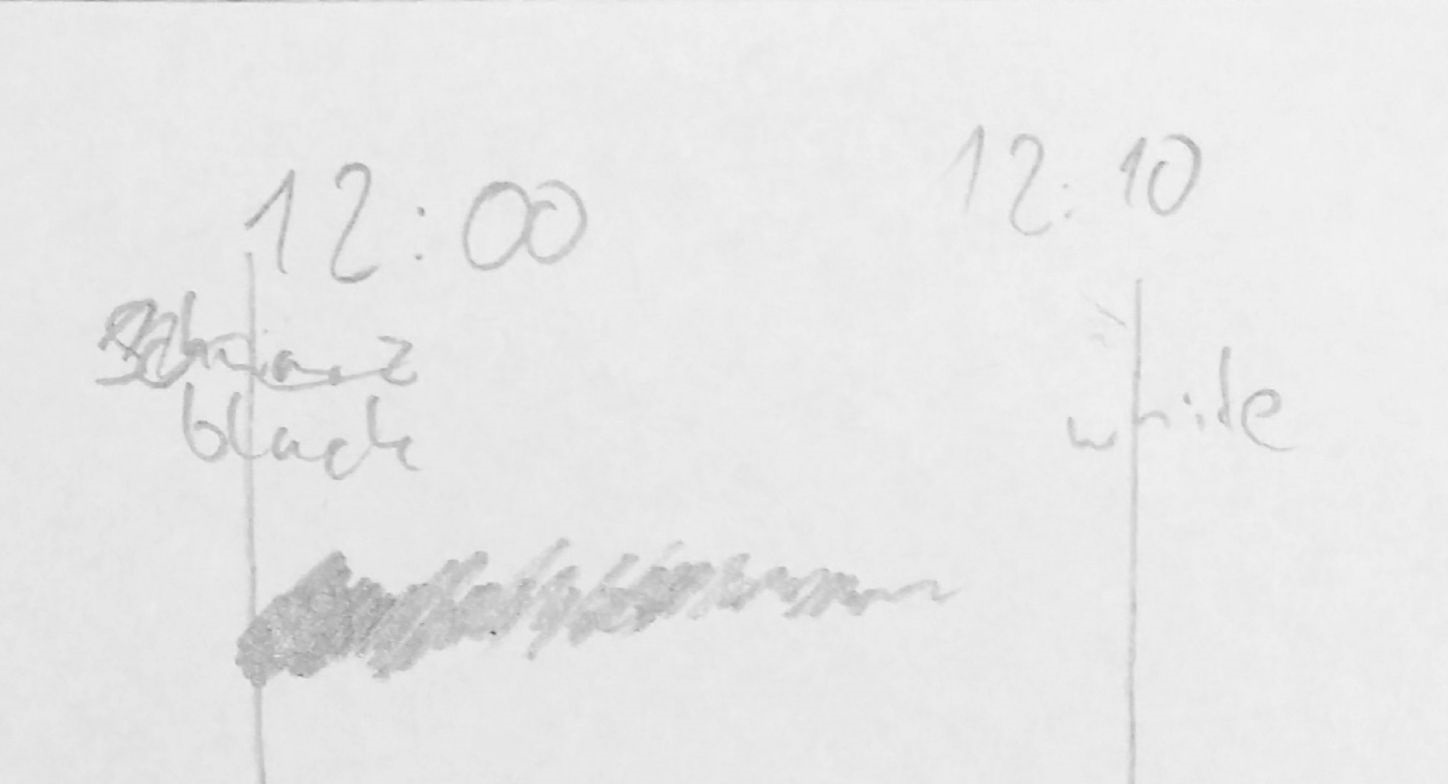
\includegraphics[width=\linewidth]{figures/color.jpg}
				\caption{\textit{The two vertical lines mark the relevant time interval. The uncertainty over this interval is given through a color gradient between those lines.}}
				\label{fig:color}
			\end{subfigure}
			
			\medskip
			
			\begin{subfigure}[t]{.4\textwidth}
				\centering
				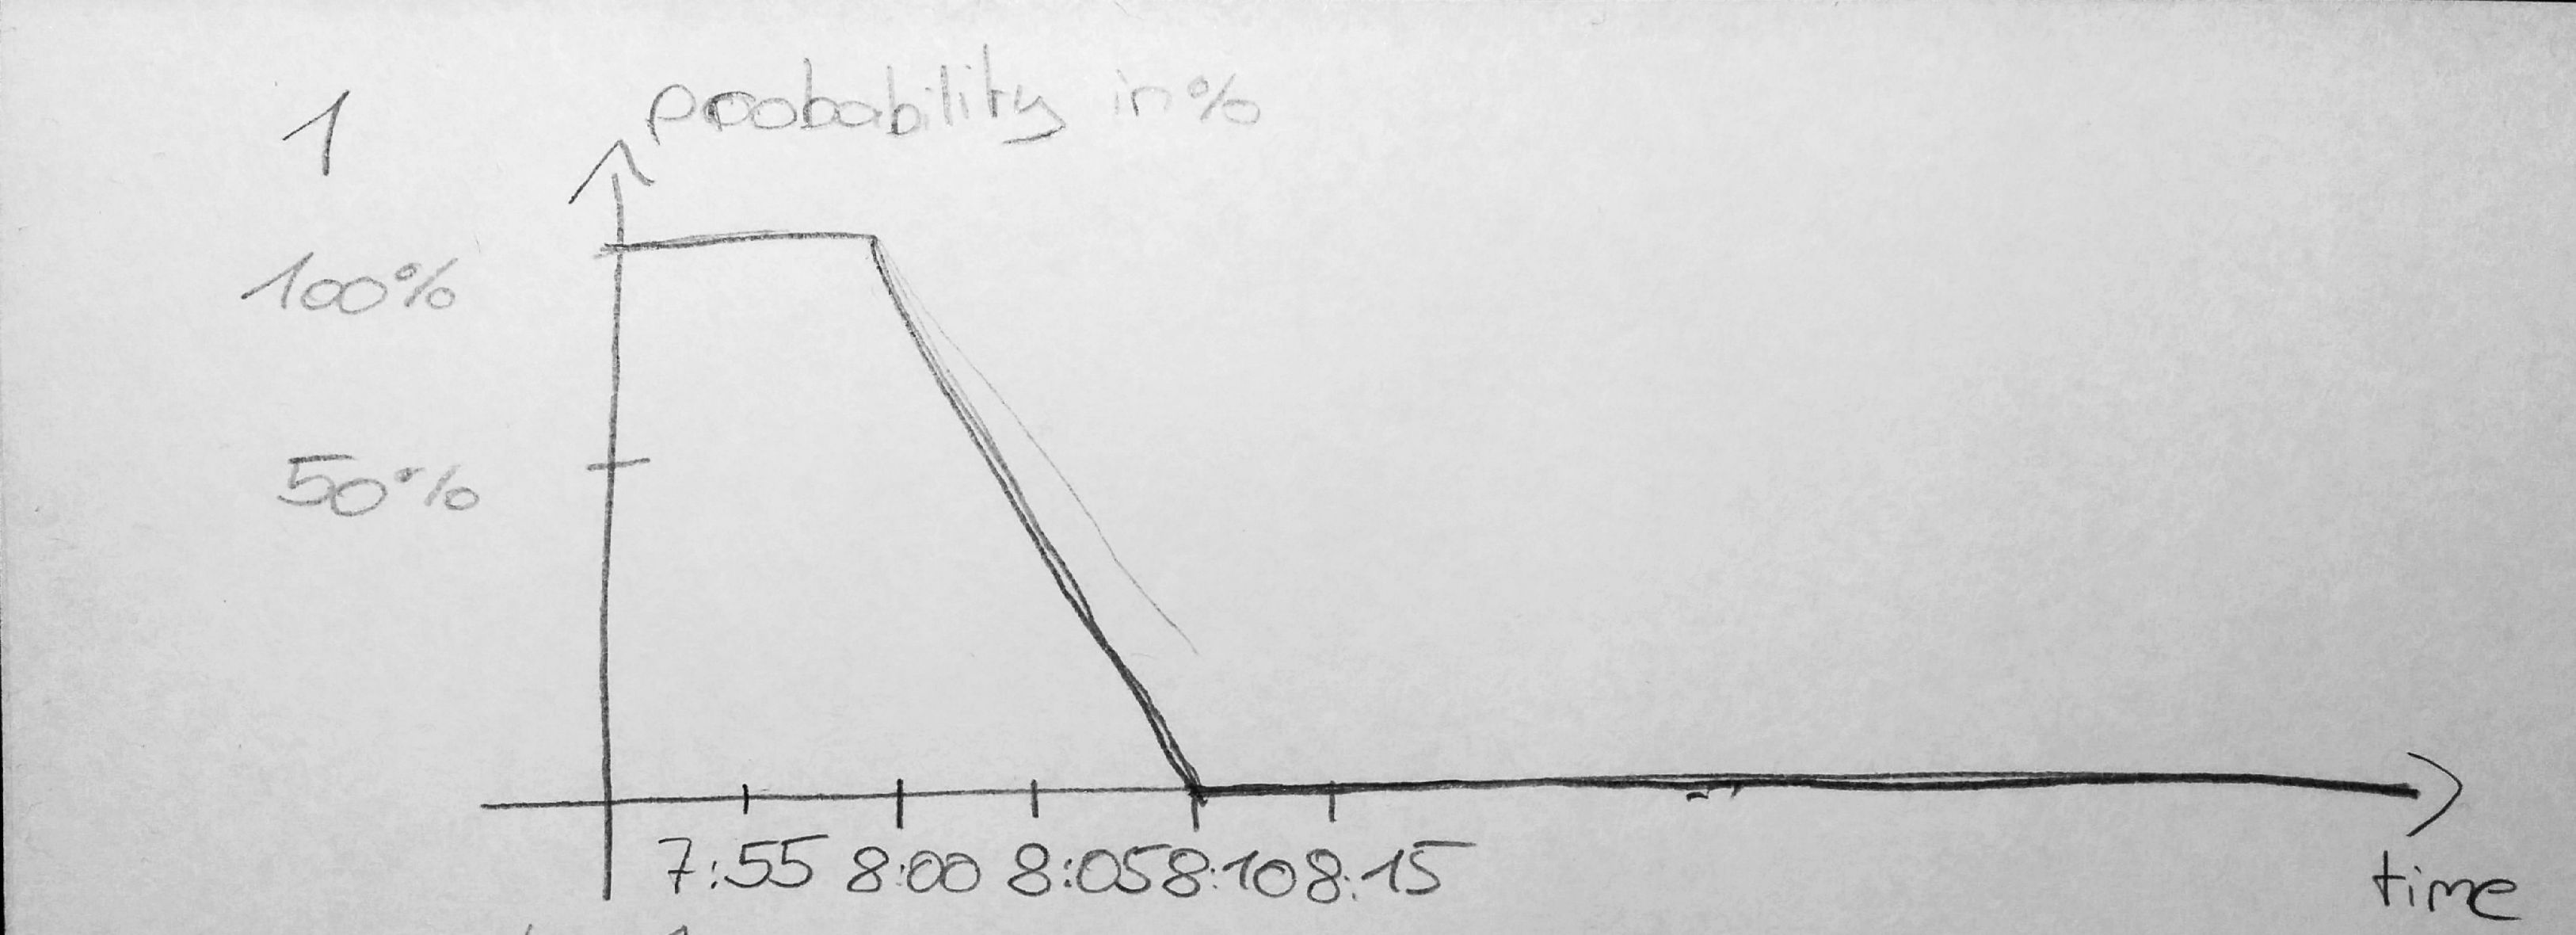
\includegraphics[width=\linewidth]{figures/length.jpg}
				\caption{\textit{This sketch shows a conventional line graph, that encoded the uncertainty over time in the height of the graph.}}
				\label{fig:length}
			\end{subfigure}
			\hfill
			\begin{subfigure}[t]{.4\textwidth}
				\centering
				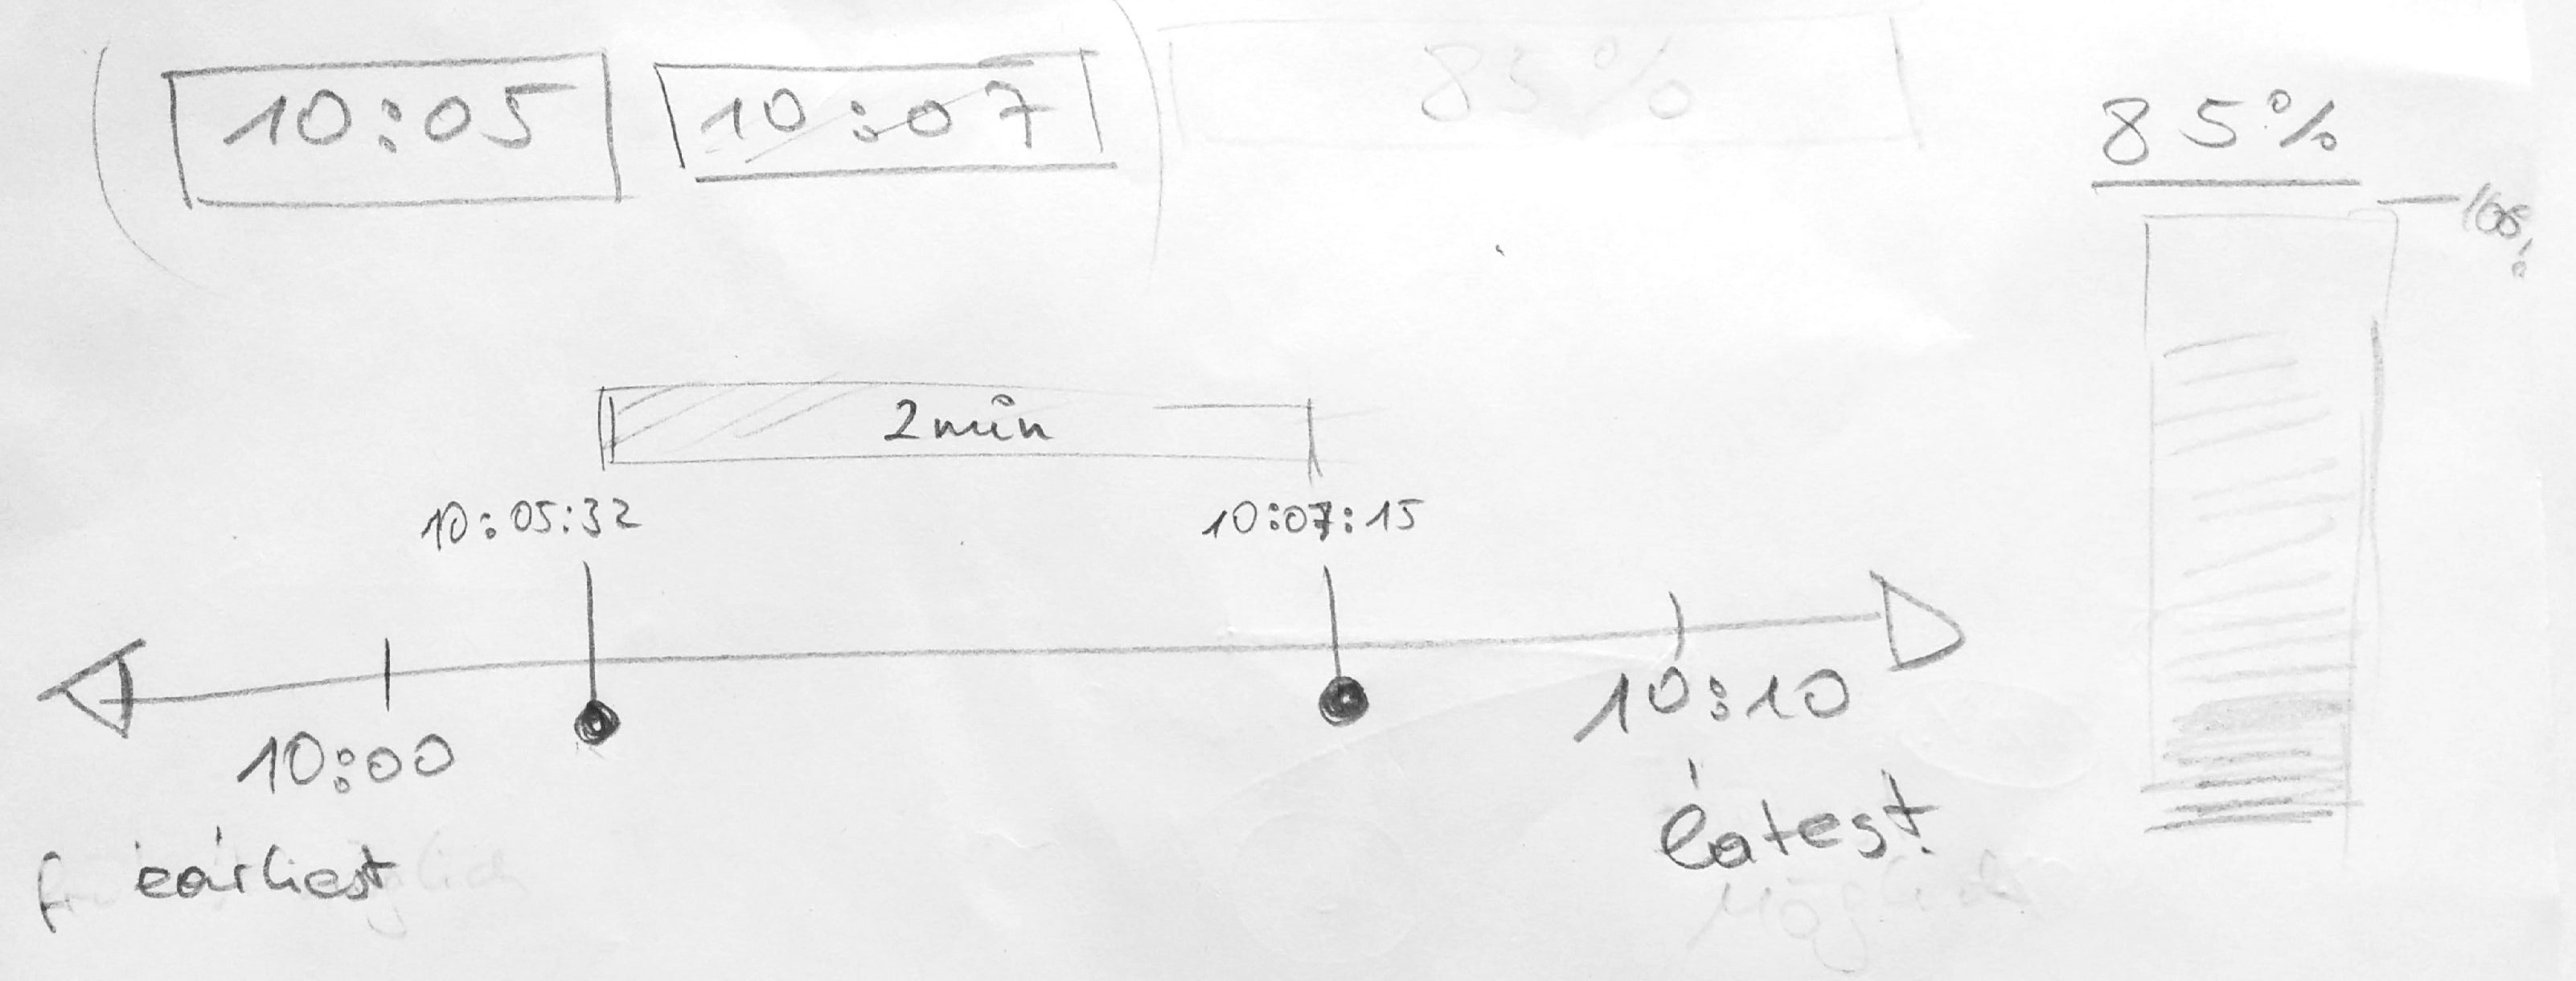
\includegraphics[width=\linewidth]{figures/interaction.jpg}
				\caption{\textit{This sketch shows an interactive visualization. The user has to pick a time interval through sliders to see the probability of catching the bus in this interval.}}
				\label{fig:interaction}
			\end{subfigure}
			\label{fig:explicit}
			\caption{\textit{The four Figures (a) through (d) show examples for the four sub-categories of explicit uncertainty representation. (a)=Icons, (b)=Color, (c)=Length/Height and (d)=interaction}}
		\end{figure}
		
		
	\end{itemize}
	\item \textbf{Bounded} If the uncertainty was not given explicitly, but only through the bounds of the uncertainty interval, the sketch counted towards this category.
	\item \textbf{Time left-right} Here we count how often there is some sort of time line from left to right, instead of any other direction.
	\item \textbf{Time top-bottom} This is the same as the last category, just from top to bottom. These two directions were chosen, because we expected them to be typical directions for time lines.
\end{itemize}

\begin{table}[h]
	\centering
	\resizebox{\textwidth}{!}{%
		\begin{tabular}{l|rr|r|lrr}
			\cline{2-7}
			\textit{\textbf{Task 1}} & \multicolumn{1}{l|}{\textbf{Graph}} & \multicolumn{1}{l|}{\textbf{Clock}} & \multicolumn{1}{l|}{\textbf{Explicit...}} & \multicolumn{1}{l|}{\textbf{Bounded}} & \multicolumn{1}{l|}{\textbf{Time left-right}} & \multicolumn{1}{l|}{\textbf{Time top-bottom}} \\ \hline
			\multicolumn{1}{|l|}{\textit{$\sum$}} & \multicolumn{1}{r|}{9} & 2 & 19 & \multicolumn{1}{l|}{11} & \multicolumn{1}{r|}{26} & \multicolumn{1}{r|}{0} \\ \hline
			\multicolumn{1}{|l|}{\textit{...Icons}} &  &  & 4 &  &  &  \\ \cline{1-1} \cline{4-4}
			\multicolumn{1}{|l|}{\textit{...Color}} &  &  & 4 &  & \textbf{} & \textbf{} \\ \cline{1-1} \cline{4-4}
			\multicolumn{1}{|l|}{\textit{...Length/Height}} &  &  & 11 &  &  &  \\ \cline{1-1} \cline{4-4}
			\multicolumn{1}{|l|}{\textit{...Interaction}} &  &  & 3 &  &  &  \\ \cline{1-1} \cline{4-4}
		\end{tabular}%
	}
	\caption{\textit{This table shows the results of the first task of the Drawing Study. The first row of numbers shows the respective counts of every category. The \textbf{Explicit...} category is further split up into its four sub-categories and their respective counts.}}
	\label{tb:t1}
\end{table}


\subsection*{Task 2 \& 3}
The results of Task 2 and 3 can be found in Table \ref{tb:t23}. It features the same categories as the table of Task 1 with two additional ones. The \textbf{Superimposed} category counts how often the two project approaches are encoded in the same space in the sketches. Figure \ref{fig:superimposed} shows an example for a superimposed representation. If the two approaches are drawn next to each other in their own space, as can be seen in Figure \ref{fig:juxtaposed}, the sketch counts towards the \textbf{Juxtaposed} category.

	\begin{figure}[H]
		\begin{minipage}{.55\textwidth}
			\centering
			\captionsetup{width=0.8\textwidth}
			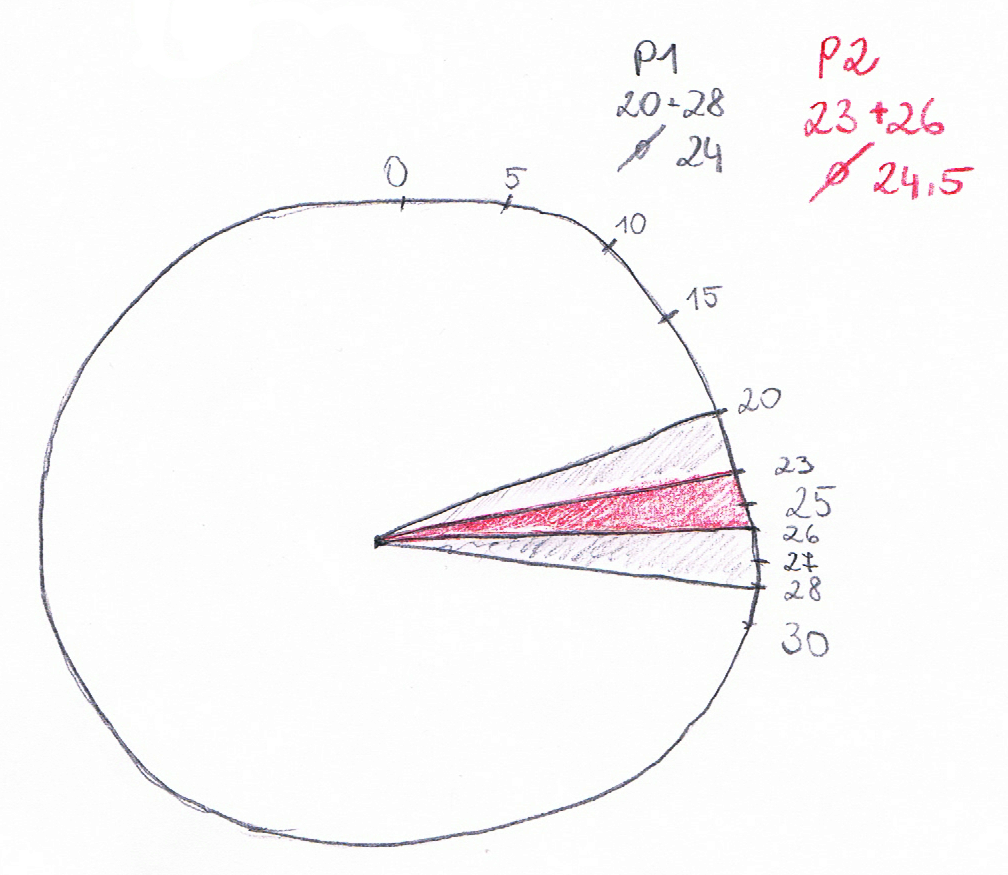
\includegraphics[height=0.5\textwidth]{figures/superimposed.png}
			\caption{\textit{This example shows the superposition of both intervals in the same clock metaphor.}}
			\label{fig:superimposed}
		\end{minipage}
		\begin{minipage}{.5\textwidth}
			\centering
			\captionsetup{width=1.0\textwidth}
			\includegraphics[height=0.5\textwidth]{figures/juxtaposed.jpg}
			\caption{\textit{As most sketches this one features a juxtaposition of the two approaches.}}
			\label{fig:juxtaposed}
		\end{minipage}
	\end{figure}

\begin{table}[h]
	\centering
	\resizebox{\textwidth}{!}{%
		\begin{tabular}{l|rr|r|lrr}
			\cline{2-7}
			\textit{\textbf{Task 2 \& 3}} & \multicolumn{1}{l|}{\textbf{Graph}} & \multicolumn{1}{l|}{\textbf{Clock}} & \multicolumn{1}{l|}{\textbf{Explicit...}} & \multicolumn{1}{l|}{\textbf{Bounded}} & \multicolumn{1}{l|}{\textbf{Time left-right}} & \multicolumn{1}{l|}{\textbf{Time top-bottom}} \\ \hline
			\multicolumn{1}{|l|}{\textit{$\sum$}} & \multicolumn{1}{r|}{5} & 1 & 17 & \multicolumn{1}{l|}{13} & \multicolumn{1}{r|}{25} & \multicolumn{1}{r|}{1} \\ \hline
			\multicolumn{1}{|l|}{\textit{...Icons}} &  &  & 0 &  &  &  \\ \cline{1-1} \cline{4-4} \cline{6-7} 
			\multicolumn{1}{|l|}{\textit{...Color}} &  &  & 5 & \multicolumn{1}{l|}{} & \multicolumn{1}{r|}{\textbf{Superimposed}} & \multicolumn{1}{r|}{\textbf{Juxtaposed}} \\ \cline{1-1} \cline{4-4} \cline{6-7} 
			\multicolumn{1}{|l|}{\textit{...Length/Height}} &  &  & 10 & \multicolumn{1}{l|}{} & \multicolumn{1}{r|}{7} & \multicolumn{1}{r|}{23} \\ \cline{1-1} \cline{4-4} \cline{6-7} 
			\multicolumn{1}{|l|}{\textit{...Interaction}} &  &  & 5 &  &  &  \\ \cline{1-1} \cline{4-4}
		\end{tabular}%
	}
\caption{\textit{This table is structured the same way as the table of Task 1 and features the results of Task 2 and 3. Additionally there are categories for superposition and juxtaposition with their respective counts.}}
\label{tb:t23}
\end{table}

\subsection*{Task 4}
The results of the fourth task are presented in the same way as the last tasks in the corresponding Table \ref{tb:t4}. Additionally, the \textbf{Superimposed} category features additional information about the use of color. Since many visualizations featured a superposition of intervals, we counted how often the two intervals were visually separated through color. This count is given in the red number next to the count of superpositions.

\begin{table}[h]
	\centering
	\begin{tabular}{l|rr|r|lrr}
		\cline{2-7}
		\textit{\textbf{Task 4}} & \multicolumn{1}{l|}{\textbf{Graph}} & \multicolumn{1}{l|}{\textbf{Clock}} & \multicolumn{1}{l|}{\textbf{Explicit...}} & \multicolumn{1}{l|}{\textbf{Bounded}} & \multicolumn{1}{l|}{\textbf{Time left-right}} & \multicolumn{1}{l|}{\textbf{Time top-bottom}} \\ \hline
		\multicolumn{1}{|l|}{\textit{$\sum$}} & \multicolumn{1}{r|}{4} & 7 & 10 & \multicolumn{1}{l|}{21} & \multicolumn{1}{r|}{23} & \multicolumn{1}{r|}{1} \\ \hline
		\multicolumn{1}{|l|}{\textit{...Icons}} &  &  & 0 &  &  &  \\ \cline{1-1} \cline{4-4} \cline{6-7} 
		\multicolumn{1}{|l|}{\textit{...Color}} &  &  & 5 & \multicolumn{1}{l|}{} & \multicolumn{1}{r|}{\textbf{Superimposed}} & \multicolumn{1}{r|}{\textbf{Juxtaposed}} \\ \cline{1-1} \cline{4-4} \cline{6-7} 
		\multicolumn{1}{|l|}{\textit{...Length/Height}} &  &  & 7 & \multicolumn{1}{l|}{} & \multicolumn{1}{r|}{22({\color[HTML]{CB0000}  11})} & \multicolumn{1}{r|}{9} \\ \cline{1-1} \cline{4-4} \cline{6-7} 
		\multicolumn{1}{|l|}{\textit{...Interaction}} &  &  & 2 & \textit{} &  &  \\ \cline{1-1} \cline{4-4}
	\end{tabular}
\caption{\textit{This table encompasses the results of Task 4. It is structured the same way as the previous tables. The individual category descriptions can be found in the list for Task 1.}}
\label{tb:t4}
\end{table}